\chapter{Grundlagen}\label{grundlagen}

Zum Verständnis dieser Arbeit ist grundlegendes Wissen nötig, welches hier in die drei Bereiche \nameref{ml-grundlagen}, \nameref{med-grundlagen} und \nameref{ballistokardiographie} unterteilt ist.


\section{Maschinelles Lernen}\label{ml-grundlagen}

Da in dieser Arbeit Methoden des Maschinellen Lernens verwendet werden, wird im Folgenden eine Übersicht über Techniken, Hintergrund und verschiedene Lernmodelle gegeben.

	\subsection{Grundprinzipien}
	
	Maschinelles Lernen ist die \glqq künstliche \grqq{} Generierung von Wissen auf Basis von Erfahrung: Aus Beispielen wird gelernt und dieses Wissen nach einer Trainingsphase verallgemeinert. Dafür wird mit Mustererkennung gearbeitet und ein statistisches Modell aufgebaut, dass auf den Trainingsdaten beruht. Die Trainingsdaten $X$ bestehen aus Merkmalsvektoren  $x \in X \subseteq \mathbb{R}^n$. Gesucht ist eine Funktion $f$, die diese Daten beschreibt. Unterschieden wird bei dieser Beschreibung dieser Daten zwischen Klassifikation. Bei einer Klassifikation werden die Eingabedaten in verschiedene Klassen unterteilt. Bei einer Regression dagegen werden stetige Werte vorhergesagt, es wird die Verteilung der Daten beschrieben. Sie kann z.B. dafür genutzt werden, Verkaufszahlen vorauszusagen. Ein Sonderfall ist die logistische Regression, die die Wahrscheinlichkeit der Angehörigkeit zu einer Klasse benennt.
	
	Es wird zwischen verschiedenen Arten des maschinellen Lernens unterschieden, dem überwachten Lernen, dem unüberwachten Lernen und dem verstärkenden Lernen. Letzteres wird hier nicht betrachtet. Bei überwachtem Lernen bestehen die vorliegenden Daten aus Eingabe-Ausgabe-Paaren $(x_1, y_1), ...,(x_n, y_n), x_i \in X$. Demnach ist nur die Funktion $f: X \to Y$ ist unbekannt. Gesucht ist eine Funktion $g$, die $f$ approximiert. Ein Lernalgorithmus ermittelt diese Funktion aus einem Hypothesenset. Dieses Vorgehen ist in Abbildung \ref{fig:supervisedLearning} visualisiert. Bei unüberwachtem Lernen dagegen ist $Y$ unbekannt; die Eingabedaten haben die Form $x_1, ..., x_n, x_i \in X$. Hier ist ein $f$ gesucht, das die Daten möglichst gut beschreibt und sie beispielsweise eigenständig in Kategorien einteilt.
	
	\begin{figure}[H]
		\centering
		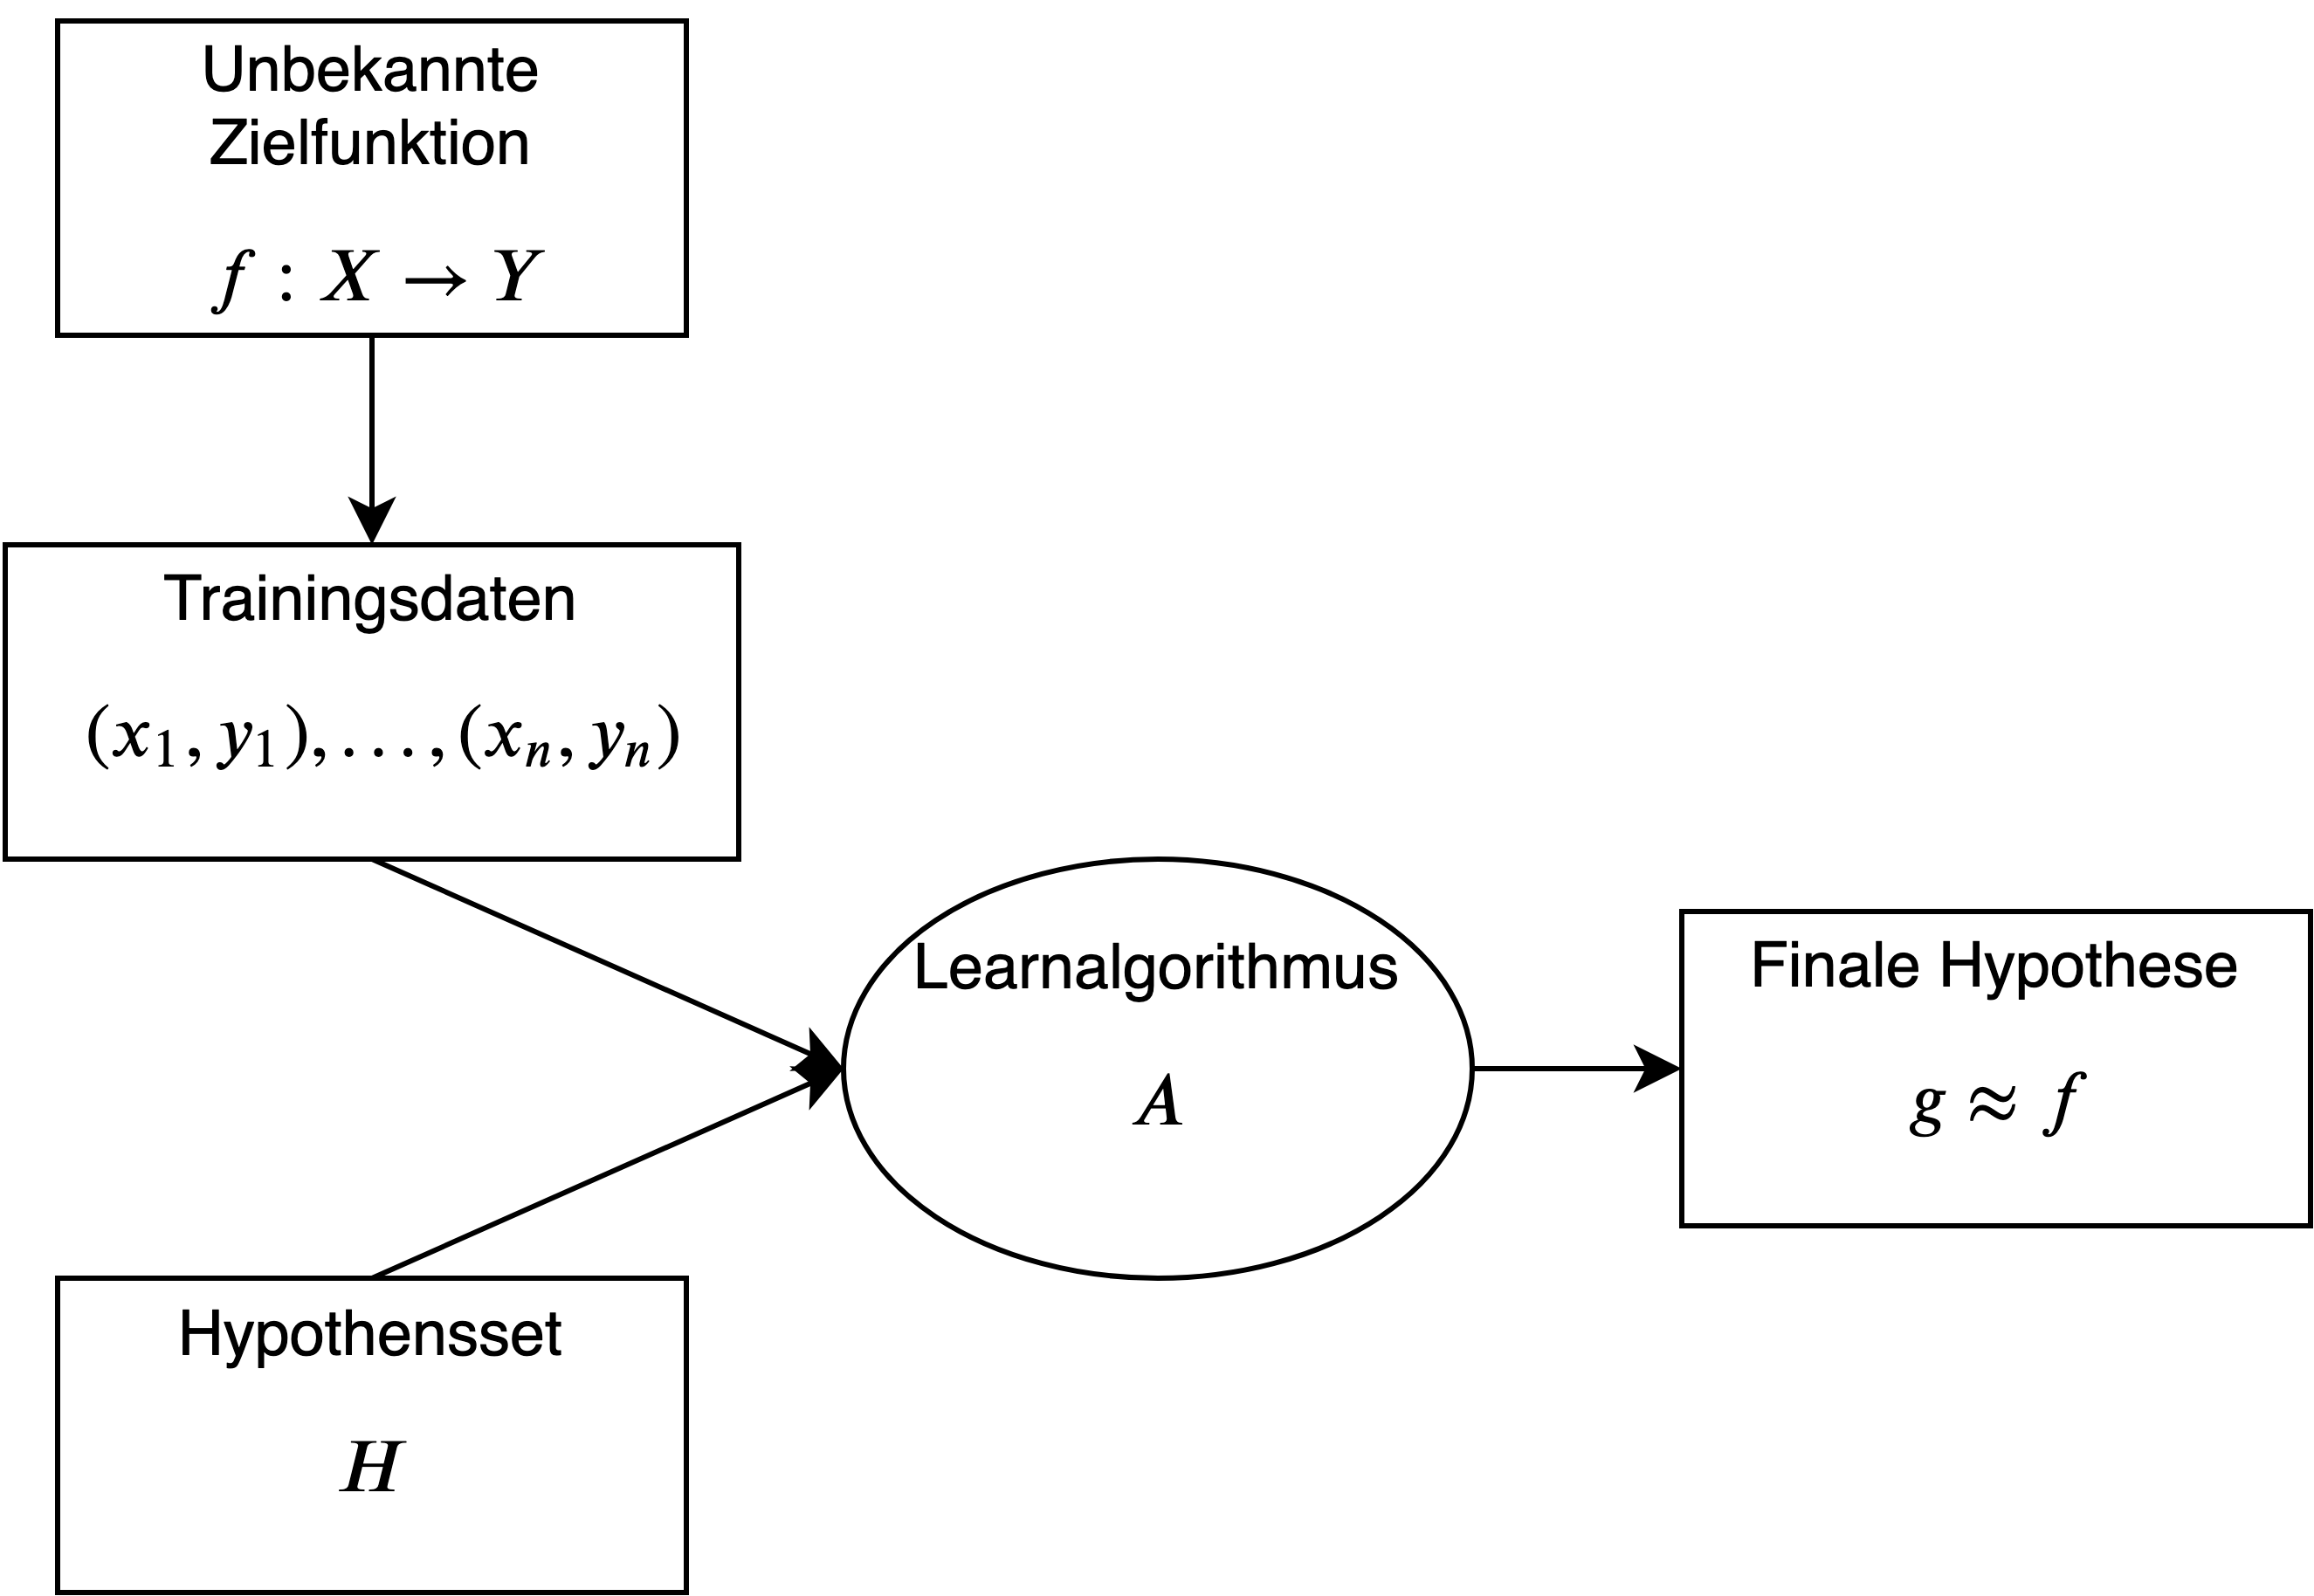
\includegraphics[width=0.7\textwidth]{pic/SupervisedLearning.png}
		\caption[Darstellung von überwachtem Lernen]{Darstellung von überwachtem Lernen}
		\label{fig:supervisedLearning}
	\end{figure}
	
	In dieser Arbeit wird überwachtes Lernen betrachtet, weshalb die untersuchten Daten annotiert werden müssen.
	
	\subsection{Mathematischer Hintergrund}
	
	\begin{itemize}
		\item auch hier nur supervised betrachtet
		\item Verteilung der Daten
		\item linear separierbar oder nicht: 3 Fälle (linear, linear mit Rauschen, nicht linear)
		\item Abbildung dazu?
		\item Ziel ist, eine Funktion zu finden, die die verschiedenen Klassen voneinander möglichst genau separiert, wodurch $y$ ermittelt werden kann bzw. bei einer Regression den Wert möglichst genau vorhersagt, Entscheidungsfunktion genannt
		\item Lineare Modelle kombinieren Merkmale linear miteinander
		\item einfachstes Modell für Klassifikation von linear separierbare Daten: Perzeptron
		\item Komponenten Merkmalsvektor x unterschiedlich gewicheten
		\item mit Gewichtungsvektor $w \in \mathbb{R}^n$
		\item Ausgabe binärer Klassifikator $y \in Y = \{-1, 1\}$
		\item Ermittlung Schwellwert \textit{Bias} $b$ mit \[
\begin{gathered}
	y = +1, \text{ falls } \sum_{i=1}^{n} w_i \cdot x_i > b \\
	y = -1, \text{ falls } \sum_{i=1}^{n} w_i \cdot x_i < b
\end{gathered}
\]
		\item wenn $w_0 = b$ und $x_0 =1$ durch Umformen Perzeptron Entscheidungsfunktion $h(x) = sign(w^Tx)$
		\item $w$ so gewählt, dass Daten korrekt klassifiziert
		\item wenn Perzeptron künstliches Neuron in Neuronalem Netz wird diese Funktion auch Aktivierungsfunktion genannt und kann variiert werden
		\item Signum Funktion hat Nachteil des "harten" Schwellwerts, oft Funktionen wie logistische Funktion mit "weichem" Schwellwert besser
		\item Lineare Regression: Gerade $h(x)$ finden, die Datenpunkte beschreibt
		\item Methode der kleinsten Quadrate, also quadratische Abweichungen zwischen Gerade und Punkten minimieren
		\item gesucht sind Koeffizienten $w$, \[\argmin_w \sum_{i=1}^{n} (w^T x_i - y_i)^2\]
		\item durch Auflösen $w = (X^T X)^{-1} X^T$
		\item bis jetzt nur lineare einfache Modelle betracht
		\item bei komplexeren Minimierungsproblemen Methode kleinster Quadrate nicht ausreichend, andere Methoden zur Fehlerminimierung -> Gradientenabstiegsverfahren
		\item graphische Vorstellung als Hügellandschaft
		\item In jedem Schritt Ableitung der Kostenfunktion nach jedem Gewicht und Bias berechnet -> Schritt wählen, der Kostenfunktion am stärksten minimiert
		\item wenn Daten nicht linear separierbar: Kerneltrick möglich
		\item Transformation (Ersetzten) des Skalarprodukts transformiert implizit den Variablenraum
		\item Beispiel Gaußscher RBF-Kernel \[K_{RBF} (x, x\prime) := exp(-\gamma \|x - x\prime\|^2) \text{ mit } \gamma > 0\]
		\item lineare Trennung in höher-dimensionalem Variablenraum
		\item Berücksichtigung aller Nicht-Linearitäten in der Transformation -> Trennfläche kann wiederum linear sein
	\end{itemize} 
	
	\subsection{Evaluation und Validierung}
	
	\begin{itemize}
		\item Modell auf unbekannten Daten validieren
		\item Hold-Out-Validierung: zufällige Verteilung in Trainings- und Testset
		\item Kreuzvalidierung
		\item Daten werden auf v gleich große Mengen (Folds) verteilt
		\item V Modelle auf allen möglichen Folds trainiert
		\item validierung auf ausgeschlossenem Fold
		\item extrem: Leave-One-Out Kreuzvalidierung mit v = n (Menge der Datenpunkte)
		\item üblich: v-fache Kreuzvalidierung
		\item typische Werte v=5 oder 10
		\item auch abhängig von verfügbarer Rechenleistung
		\item Wofür
		\item Schätzung von Fehler auf unbekannten Daten
		\item Wahl von Modellen/Bestimmung von Hyperparametern
		\item Parameter, die Modellarchitektur bestimmen
		\item Parameter, die Lernalgorithmus betreffen
		\item Regularisierungsparameter
		\item Ergebnis: 3 Datensets
		\item training, validierung, test
		\item Validierungsset beeinflusst Lernalgorithmus
		\item Testset nachdem alle Entscheidungen getroffen wurden
		\item typisch: Validierung durch zB Kreuzvalidierung auf Testset
		\item Retraining auf ganzem Trainingsset
		\item Ablaufdiagramm
		\item dafür evaluationsmetrik nötig -> Übergang
		\item verschiedenste Metriken
		\item begriffe TP, FP, TN, FN
		\item Accuracy $ACC = \frac{TP + TN}{TP + TN + FN + FP}$ einfaches Gütemaß, problematisch bei ungleich großen Klassen, da eine hohe Genauigkeit erreicht wird, wenn immer die größere Klasse vorausgesagt wird
		\item Precision, "bestraft" Falsch-Positive $PPV = \frac{TP}{TP + FP}$
		\item Recall, auch Sensitivity genannt, "bestraft" Falsch-Negative $TPR = \frac{TP}{TP + FN}$
		\item Oft Recall und Precision in einem Maß zusammengefasst: F1 score harmonisches Mittel aus beiden $F_1 = 2 * \frac{precision * recall}{precision + recall}$
		\item nicht balancierte Datensets
		\item balanced accuracy
		\item roc kurz für Receiver Operating Characteristic. basiert auf True Positive Rate TPR und False Positive Rate FPR, charakterisiert, wie gut beide Verteilungen durch Schwellwert trennbar sind
		\item auc Fläche unter der ROC Kurve
	\end{itemize}
	
	\subsection{Probleme maschinellen Lernens}
				
		\begin{itemize}
			\item offensichtich: Underfitting
			\item Overfitting -> gute Approximation aber schlechte Generalisierung auf unbekannte Daten
			\item Einfluss von: Komplexität des Lernmodells, Datenmenge, Kontamination der Daten mit Rauschen
			\item mehr Datenpunkte mehr gut, Rauschen und Komplexität schlecht
			\item TODO: Bild
			\item Regularisierung gegen Overvitting: TODO näher nachlesen
			\item Stichprobenverzerrung
		\end{itemize}

	\subsection{Weitere Lernmodelle des Überwachten Lernens}
	
		\subsubsection{Entscheidungsbäume}
		
		\begin{itemize}
			\item Bild mit Thresholds und Features
			\item an jedem Knoten Entscheidung ob bestimmtes Feature über Threshold liegt
			\item generiert z.B. durch rekursives binäres Teilen
			\item bei Regression mittlere quadratische Abweichung $MSE$ minimieren, bei Klassifikationsbäumen Messung der "Unreinheit" der Blätter (Fehler = 0 wenn Blatt nur Punkte derselben Klasse, Fehler maximal wenn keine Klasse Mehrheit)
			\item Optimierung rechnerisch nicht effizient lösbar
			\item greedy den Schritt, also die Kombination aus Feature und Threshold wählen, der den Fehler am Stärksten reduziert
			\item Abbruchkriterien: maximal erlaubte Tiefe, Mindestanzahl Datenpunkte in einem Blatt
			\item keine Featureskalierung nötig
		\end{itemize}
		
		\subsubsection{Random Forest}
		
		\begin{itemize}
			\item besteht aus mehreren unkorrelierten Entscheidungsbäumen
			\item Randomisierung bei Erstellung der Bäume
			\item Mehrheitsentscheidung aller Bäume
			\item Nach Breiman für jeden Baum im Wald
			\item n Bootstrap Samples ziehen, also mit Zurücklegen aus dem Trainings-Datensatz gezogen
			\item von $M$ Merkmalen $m \ll M$ Merkmale zufällig gewählt, die als Kriterium für Split infrage kommen
			\item voller Ausbau des Baums
		\end{itemize}
		
		
		\subsubsection{Nächste Nachbarn Modelle}
		
		\begin{itemize}
			\item sehr einfache Modelle, öfters zur Schätzung einer Baseline im Einsatz
			\item Klassifikation anhand der Datenpunkte, die zu klassifierenden Datenpunkt am nächsten liegen
			\item dafür Ähnlichkeit quantifizieren
			\item kein Training, Modell direkt durch Trainingsdaten definiert
			\item Voronoi-Regionen werden erzeugt: Menge aller Punkte die näher an einem Zentrum liegen als an allen anderen Zentren
			\item daraus Voronoi-Diagramm (gesammelte Grenzen)
			\item k-Nächste Nachbarn: das Label der Mehrheit der k nächsten Punkte wird zurückgegeben
			\item Regression: Mittelwert-Bildung über die Label der k nächsten Nachbarn
		\end{itemize}
		
		\subsubsection{Support Vector Machines}
		
		\begin{itemize}
			\item Rauschen in Daten
			\item statt einfache Gerade wie bei Perzeptron wird Hyperebene mit maximalem Rand gesucht, die Daten korrekt klassifiziert
			\item TODO: Bild von Gerade mit Rand
			\item Ausgangspunkt Perzeptron, Umformulierung in Optimierung mit Nebenbedingung, dass Hyperebene größten Rand besitzt
			\item bei SVMs oft oben schon erwähnter Kernel-Trick, also Transformation des Skalarprodukts, damit nicht-lineare Separierung möglich
		\end{itemize}
		
		\subsubsection{Mehrlagiges Perzeptron}
		
		\begin{itemize}
			\item Klasse von künstlichen neuronalen Netzwerken
			\item 3 Schichten: Eingabe-Schicht, Versteckte Schicht, Ausgabe-Schicht
			\item außer den Eingabeneuronen wird nicht-lineare Aktivierungsfunktion verwendet
		\end{itemize}


\section{Medizinische Grundlagen}\label{med-grundlagen}

Die vorliegende Arbeit beschäftigt sich mit der Beurteilung der Signalqualität in ballistokardiographischen Signalen. Zum Verständnis der gemessenen Vorgänge und der Problematik in Bezug auf die Signalqualität und dessen Beurteilung ist grundlegendes medizinisches Wissen über die gemessenen Vorgänge und messtechnisches Verständnis nötig. Aufgrund dessen wird hier eine kurze Übersicht über die medizinischen Grundlagen gegeben.

	\subsection{Kardiorespiratorisches System}
	
	Das kardiorespiratorische System (zusammengesetzt aus \textit{kardìa}, deutsch \textquoteleft Herz\textquoteright und \textit{respiratio}, deutsch \textquoteleft Atmung\textquoteright) setzt sich aus zwei Teilsystemen zusammen, dem kardiovaskulären und dem respiratorischen System, die zusammen die Versorgung der Organe mit sicherstellen.
	
	Das kardiovaskuläre System umfasst das Herz, die Arterien und die Venen. In einem Zyklus wird das sauerstoffreiche Blut von der linken Herzkammer durch die Arterien zu den Organen gepumpt, wo sich der Sauerstoff zur Versorgung dieser vom Blut löst. Die Venen transportieren das nun kohlstoffdioxidreiche Blut in die rechte Herzkammer. Von dort wird es zur Lunge geführt, mit Sauerstoff angereichert und in die linke Herzkammer geleitet. Von dort beginnt der Vorgang von Neuem. Die Herzfrequenz ist hierbei ein relevanter messbarer Vitalparameter.
	
	Ein Herzschlag selbst besteht aus zwei Phasen: einer füllenden und einer auswerfenden Phase. Während der Diastole, der Erschlaffungs- und Bluteinströmungsphase, füllen sich die Herzkammern mit Blut. Diese Phase endet mit dem Schließen der Herzklappen und die Systole beginnt. Die Systole ist die Anspannungs- und Blutausströmungsphase: Die Herzklappen öffnen sich durch Kontraktion des Herzmuskels und das Blut kann ausströmen.
	
	Das respiratorische System umfasst die Lungen und den Lungenkreislauf. In einem Atemzyklus wird durch gezielte Muskelbewegungen Luft aus der Umgebung eingeatmet. Mit dem eingeatmeten Sauerstoff wird sauerstoffarmes Blut angereichert und anschließend die nun sauerstoffarme Luft ausgeatmet. In diesem Zusammenhang ist der Vitalparameter der Atemfrequenz messbar.

	\subsection{Übersicht Messtechniken}
	
	Zur Untersuchung der in dieser Arbeit betrachteten \acf{BKG} wird diese oft mit anderen Messmethoden als Referenz aufgenommen. Im Folgenden werden diese zur Einordnung kurz vorgestellt. \ac{BKG} selbst wird im nächsten Abschnitt separat betrachtet.
	
	Die \acf{EKG} zeichnet die elektrischen Aktivitäten des Herzmuskels auf, indem mit mehreren Elektroden die Spannungsänderung gemessen wird. Hier ist die Herzfrequenz sehr gut ablesbar.
	
	Die \acf{PPG} ist ein optisches Messverfahren, bei dem die Menge des von der Haut reflektierten bzw. transmittierten Lichtes gemessen wird. Dadurch kann die Änderung des Blutvolumens gemessen werden; die Lichtmenge nimmt bei Durchlaufen einer Pulswelle durch die Arterie deutlich ab. Dieses Signal bietet Rückschluss auf Atmung und Herzschlag. % TODO: evtl. reinnehmen
	
	Oft gemeinsam mit dem \ac{BKG} betrachtet wird die \acf{SKG}, bei der die Vibration der Wand des Brustkorbs, die durch den Herzschlag entsteht, aufgezeichnet wird. Aufgrund von fehlenden einheitlichen Definitionen wird in der Literatur teils auch der Begriff \ac{BKG} für \ac{SKG} genutzt.\footcite[Vgl.][]{Inan2015}

	\section{Ballistokardiographie}\label{ballistokardiographie}
	
	Im Folgenden wird die \acl{BKG} eingeführt. Das beinhaltet den medizinischen und technischen und Hintergrund, das Einsatzgebiet und die Signaleigenschaften.
	
	\subsection{Medizinischer und technischer Hintergrund}
	
	Ballistokardiographie (zusammengesetzt aus altgriechisch \textit{ballein}, deutsch \textquoteleft werfen\textquoteright, \textit{kardía}, deutsch \textquoteleft Herz\textquoteright und \textit{graphein}, deutsch \textquoteleft schreiben\textquoteright) ist die graphische Darstellung der wiederholten, durch den Herzschlag verursachten Bewegungen des menschlichen Körpers. Erstmals schon im 19. Jahrhundert beobachtet\footcite[Vgl.][]{Gordon1877}, ermöglicht der technische Fortschritt in der Sensortechnik heute aussagekräftige Messungen. Das \ac{BKG} liefert durch die Aufzeichnung von zirkulierendem Blut und mechanischer Herzaktivität Informationen über die Gesamtleistung des kardiovaskulären Systems.\footcite[Vgl.][]{Pinheiro2010} Konkret gemessen wird eine Massenbewegung, die durch die schnelle Beschleunigung des Blutes entsteht, wenn es während des Herzschlages durch die großen Arterien bewegt wird: Bei der Verteilung des Blutes in die peripheren Blutgefäße verschiebt sich das Zentrum der Körpermasse in Richtung der Füße und während der atrialen Systole Richtung Körpermitte. Die \ac{BKG}-Wellenform entsteht durch diese Schwerpunktverschiebung.
	
	Die Messung dieser Bewegung ist mit verschiedenen Sensortypen, die z.B. hydraulisch oder elektromechanisch auf Druck reagieren, möglich. Sensoren können unter anderem in Waagen, Stühlen und Betten eingebaut werden. Besonders bei im Bett gemessenen Signalen kann oft nicht klar zwischen \ac{SKG} und \ac{BKG} unterschieden werden, da sich myokardiale Vibrationen und Massverschiebungen durch den Blutfluss überlagern. Diese gemischten Signale werden in der Literatur teils auch als \textit{cardiac vibration signals} bezeichnet.\footcite[Vgl.][]{Bruser2013} Da im Bereich der Signalverarbeitung oft nicht zwischen reinem \ac{BKG} und gemischten Signalen unterschieden wird, wird dies in der vorliegenden Arbeit ebenfalls nicht.
	
	Verschiedene Studien kommen zu unterschiedlichen Ergebnissen bezüglich der Frage, welchen kardiovaskulären Ursprung die einzelnen Signalteile haben. Aufgrund dessen gestaltet sich die detaillierte Interpretation des \ac{BKG}-Signals als schwierig. Da es neben Informationen zur \ac{HR} und \ac{HRV} ein genauerer Indikator für das Alter des Herzens als Lebensalter ist, hat es trotzdem klinische Relevanz. Außerdem lassen sich durch abnormale Ballistokardiogramme Herzerkrankungen voraussagen, bevor Symptome auftreten. Besonders bei älteren Personen sind diese also eine wichtige Warnung.\footcite[Vgl. zu diesem Absatz][]{Pinheiro2010}
	
	\subsection{Einsatzgebiet}
	
	Durch diese Beschreibung wird schon deutlich, dass \ac{BKG} anders als das sehr bekannte \ac{EKG} ist. Der entscheidende Vorteil des \ac{BKG}s liegt darin, dass kein einschränkender Körperkontakt wie z.B. durch aufgeklebte Elektroden nötig ist: Es lässt sich in Alltagsgegenständen wie Stühlen aber vor allem auch Betten implementieren, ohne dass es während der Messung zu Einschränkungen im alltäglichen Leben kommt oder medizinisches Fachpersonal anwesend sein muss. Damit gehört es zu den \textit{unobtrusive} Messmethoden und eignet sich gut zur Langzeit- und Trendbeobachtung des Gesundheitszustandes - sowohl im klinischen Kontext als auch Zuhause. Besonders für Patient*innen mit chronischen Krankheiten und zur Früherkennung krankhafter Veränderungen bietet eine gesundheitliche Überwachung von Zuhause großes Potential.\footcite[Vgl.][]{Inan2015} Je nach Aufbau des Messsystems verändert sich auch die Art der Informationen, die aus dem \ac{BKG}-Signal gewonnen werden können. Sehr genaue, kontrolliert aufgenommene \ac{BKG}-Signale ermöglichen eine aussagekräftige Analyse der Morphologie wobei beispielsweise in Betten eingebautes \ac{BKG} zunächst nur Aussagen zu Herzrate und Herzratenvariabilität bietet. Zusätzlich zu Informationen der Herzaktivitäten ermöglichen Bettsysteme aber auch Informationen über das allgemeine Aktivitätslevel und somit auch über die Schlafqualität. \footcite[Vgl.][]{Bruser2011} In dieser Arbeit wird es um die Aufzeichnung von \ac{BKG}-Signalen in Betten gehen. Der Aufbau eines solchen Bettsystems ist in Abbildung \ref{fig:bcgbed} gezeigt.
	
	 \begin{figure}[H]
	 	\centering
		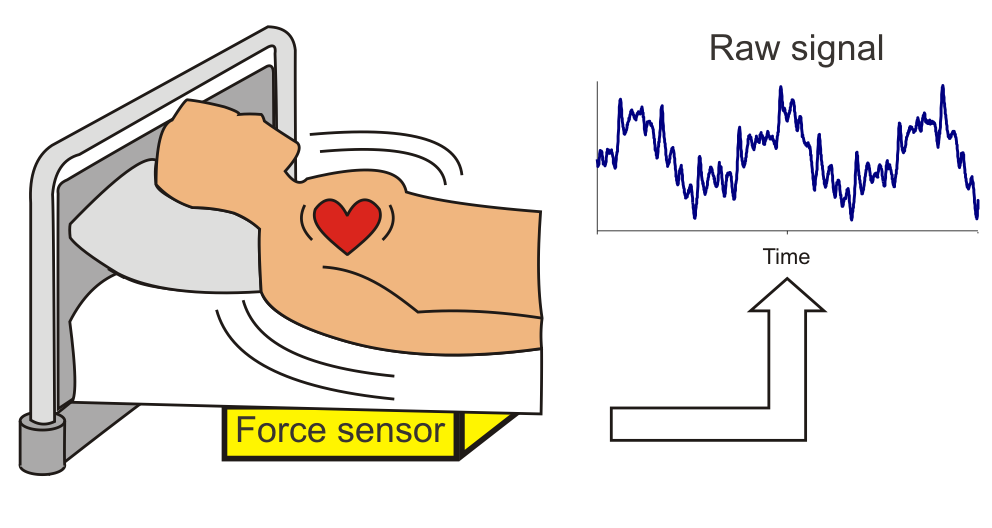
\includegraphics[width=0.5\textwidth]{pic/bcgBed.png}
		\caption[Übersicht über die Funktionsweise eines allgemeinen im Bett eingebetteten \ac{BKG}-Systems]{Übersicht über die Funktionsweise eines allgemeinen im Bett eingebetteten \ac{BKG}-Systems.\protect\footnotemark}
		\label{fig:bcgbed}
	\end{figure}
	\footnotetext{Entnommen aus \cite{Bruser2011}}
	
	Allerdings ergeben sich neben diesen umfassenden Möglichkeiten auch Nachteile gegenüber konventionellen Messmethoden. Die größte Herausforderung ist eine stark variierende Signalqualität, die sich durch das unkontrollierte Umfeld und die Art der Messung ergibt.

	\subsection{Signaleigenschaften}
	
	Das gemessene \ac{BKG}-Signal setzt sich aus Herzaktivitäten, Atmungsaktivitäten und Körperbewegungen zusammen. Gegebenenfalls wird es noch durch Störungen der Messung beeinflusst. Bei einer gesunden Person ohne Störeinflüsse wird die in Abbildung \ref{fig:bcgwaveform} abgebildete Wellenform erwartet. Diese Idealform lässt sich in 3 Gruppen unterteilen: Die präsystolische, wobei diese häufig nicht beachtet wird, die systolische und die diastolische Gruppe unterteilen. Die mit H bis K markierten Extremwerte gehören bei dieser Unterteilung zur systolischen Gruppe, die Wellen L bis N zur diastolischen Gruppe. Die präsystolische Gruppe, die aus den Wellen F und G besteht, ist in hier nicht abgebildet. I und J werden auch als \textit{ejection waves} bezeichnet. In Bezug auf andere Messmethoden ist zu bemerken, dass die H-Welle nahezu synchron mit dem ersten Herzgeräusch ist. Der Abstand des R-Peaks, des Hochpunkts eines \ac{EKG}s zur H-Welle variiert im Bereich von 0,2 bis 0,3 Sekunden.\footcite[Vgl.][]{DELALLA1950} Die Amplitude der Wellen ohne Störeinflüsse ist hauptsächlich abhängig von dem Herzzeitvolumen, der Herzkraft und der Geschwindigkeit des Auswurfs.\footcite[Vgl.][]{Pinheiro2010}
	
	\begin{figure}[H]
		\centering
		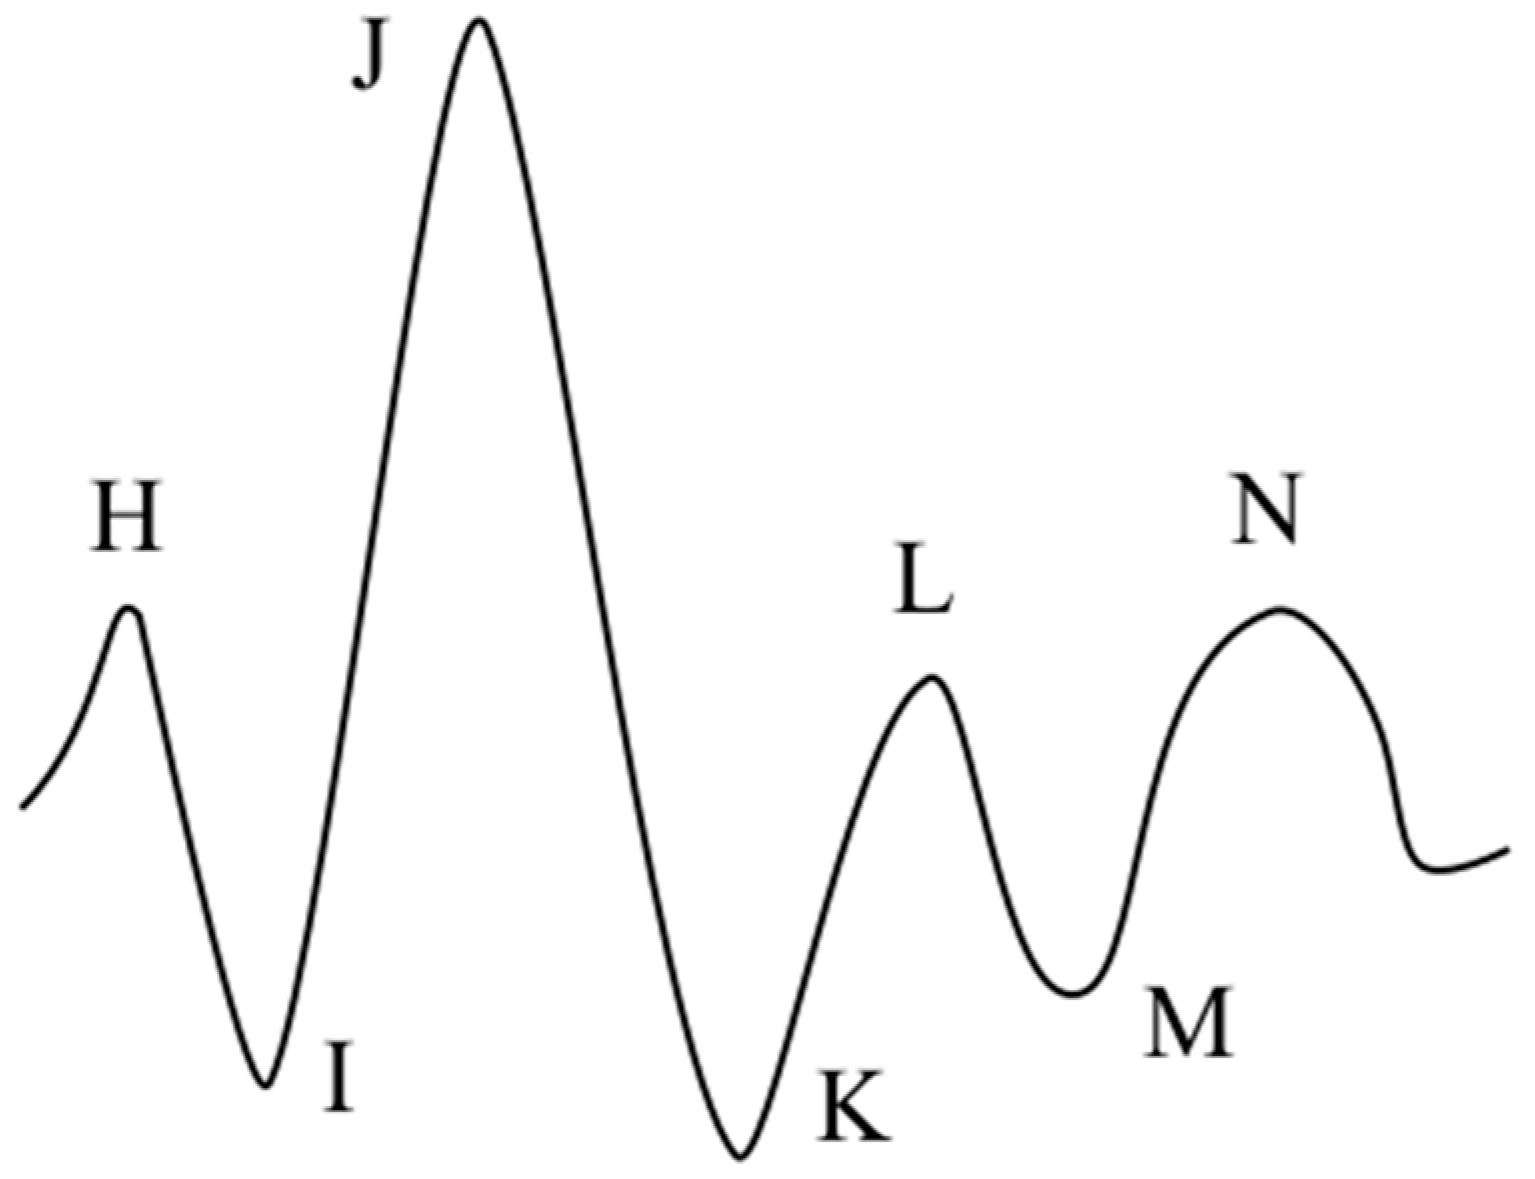
\includegraphics[width=0.5\textwidth]{pic/bcgWaveform.png}
		\caption[Beispiel eines typischen \ac{BKG}-Signals mit Nomenklatur]{Beispiel eines typischen \ac{BKG}-Signals mit Nomenklatur\protect\footnotemark}
		\label{fig:bcgwaveform}
	\end{figure}
	\footnotetext{Entnommen aus \cite{Albukhari2019} nach \cite{Starr1939}.}
	
	Im Idealfall wird zwar die oben beschriebene Wellenform erwartet, bei der die Wellen H bis L eine deutliche W-Form bilden, allerdings ist es trotz dieser typischen Form selten, dass alle nicht-systolischen Komponenten sichtbar sind.\footcite[Vgl.][]{Pinheiro2010} Es gibt eine starke Variation der Signalmorphologie sowohl zwischen als auch innerhalb von Individuen. Der größte Einfluss ergibt sich durch die verwendeten Sensoren und die Position der Person, also zum Beispiel ob im Stehen, Sitzen oder Liegen gemessen wird.\footcite[Vgl.][]{Sadek2019} Es gibt Studien die zeigen, dass die intraindividuelle Varianz über serielle Messungen hinweg niedrig ist.\footcite[Vgl.][]{Inan2015} Allerdings gilt das nicht, wenn sich die Position der Person verändert. Hierbei reicht es schon, wenn die Person in Rückenlage statt Seitenlage liegt.\footcite[Vgl.][]{Bruser2011} Aufgrund dieser Variationen in der Signalmorphologie wurden schon in den 1950er Jahren 3 Achsen für die Aufzeichnung des \ac{BKG}s definiert: Die longitudinale (Kopf-Fuß), die transversale (Seite-Seite) und die dorsoventrale (Rücken-Brust).\footcite[][Vgl.]{Bruser2011, Inan2015} Zu Beginn maßen die meisten Systeme entlang der longitudinalen Achse, die z.B. der Messung auf einer Waage entspricht. \textit{Unobtrusive} Messsysteme, wie die hier betrachtete Messung in Betten, messen entlang einer Kombination der transversalen und der dorsoventralen Achse - abhängig von der Position der Person. Besonders diese Kombination sorgt für eine große intra- und individuelle Variation des Signals. Abbildung \ref{fig:bcg2postures} verdeutlicht dies durch den direkten Vergleich von \ac{BKG}-Aufzeichnungen zweier Herzschläge von 2 Personen. Bei jedem Probanden wurde in zwei verschiedenen Positionen gemessen.\footcite{Bruser2011} Auch der Ursprung des Signals ist abhängig von der Messachse. Bei longitudinale gemessenem \ac{BKG} ist der Einfluss des Herzzeitvolumens schon seit 1929 beobachtet.\footcite[Vgl.][]{Starr1939} Im Gegensatz dazu ist der Ursprung des in Betten gemessenen \ac{BKG}-Signals nicht genau bekannt. Das liegt unter anderem daran, dass mechanische Komponenten wie z.B. die Matratze einen schwer zu modellierenden Einfluss haben.
	
	\begin{figure}[H]
		\centering
		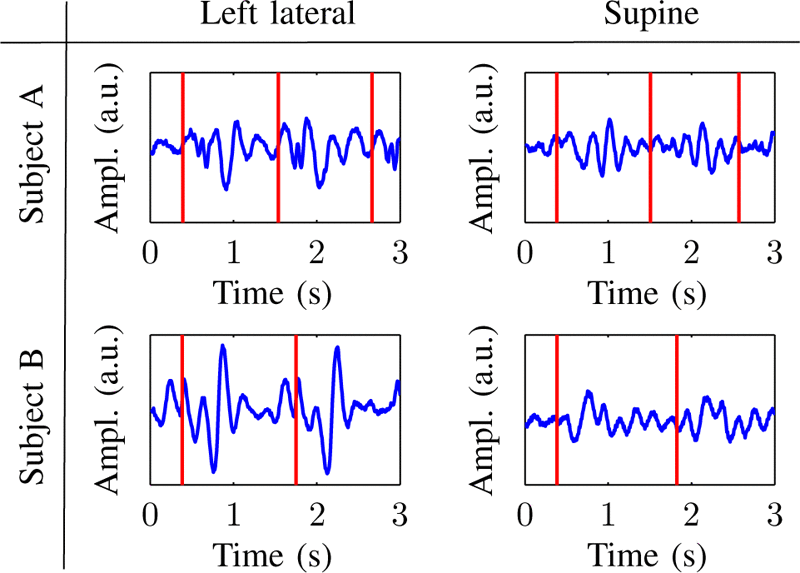
\includegraphics[width=0.5\textwidth]{pic/bcg2postures.png}
		\caption[\ac{BKG}-Aufnahmen in Rücken- und Seitenlage]{Hochpass-gefilterte \ac{BKG}-Aufnahmen von zwei Herzschlägen zwei verschiedener Personen, jeweils in Rücken- und Seitenlage gemessen. Die vertikalen Linien markieren die R-Peaks der EKG-Referenz.\protect\footnotemark}
		\label{fig:bcg2postures}
	\end{figure}
	\footnotetext{Entnommen aus \cite{Bruser2011}.}
	
	Neben Einflüssen der verwendeten Messachse und der Körperposition beeinflusst auch die Atmung die Signalform. Normale Atmung beeinflusst die Amplitude der \textit{ejection waves} I und J. Bei Atemstillstand dagegen werden die H und J Wellen verzerrt. Auch bei einer gesunden, sich nicht bewegenden Person, die ihre Atmung kontrolliert, wird kein exakt Schlag für Schlag reproduzierbares Signal erzeugt werden.\footcite[Vgl.][]{Pinheiro2010} Von \citeauthor{Zink2017} werden die Einflüsse der Atmung in der vertikalen Achse eines dorsoventralen \ac{BKG}s als große Schwingungen einer Wellenlänge von fünf bis zehn Sekunden beschrieben. Innerhalb dieser sind kleinere Schwingungen mit höherer Frequenz sichtbar, die jedoch keiner bestimmten Sequenz folgen.\footcite[Vgl.][]{Zink2017} Zusätzlich zu dieser schon beschriebenen Variabilität kommt es sehr leicht zum Entstehen von Artefakten. Ursprung ist entweder das Messsystem selbst oder Körperbewegungen. Insgesamt führt Bewegung der Patient*innen, auch die der Atmung, zu einem \textit{baseline drift}. Stärkere Bewegungen führen zu einer Massenverschiebung, die um ein Vielfaches größer als die gemessenen Vorgänge ist. Aufgrund dessen führt sie immer dazu, dass das Signal stark verzerrt oder sogar vollständig überlagert wird.

	
	Besonders im Vergleich zu anderen kardiorespiratorischen Signalen wie dem \ac{EKG} und \ac{PPG} wird deutlich, dass \ac{BKG}-Signale auch in konsekutiven Messungen deutlich variabler sind. Abbildung \ref{fig:variabilitaet} zeigt dies am Beispiel von \ac{BKG}-Aufnahmen eines im Bett integrierten Messsystems im Vergleich zum parallel aufgenommenen \ac{EKG}. Es zeigt sich, dass selbst nach Entfernung von Überlagerungen von Atmung  und Bewegung das \ac{BKG}-Signal eine höhere Variabilität in Bezug auf Amplitudenhöhe, Reihenfolge der Extremwerte und der gesamten Form aufweist.\footcite[Vgl.][]{Zink2017} Es wird allerdings angenommen, dass aufeinander folgende Herzschläge sich ähneln. Diese Eigenschaft wird Selbstähnlichkeit genannt. \citeauthor{Bruser2013} nennt als eine mögliche Ausnahme den Fall, dass ein unregelmäßiger Herzschlag mit sehr niedrigem Schlagvolumen einem regulären Herzschlag folgt. In dem Fall ist es möglich, dass die Amplitude im Vergleich so klein ist, dass sie verdeckt wird. Dies ist z.B. bei Vorhofflimmern möglich. Eine Untersuchung von \citeauthor{Rosales2012} zeigt dieses Verhalten der Selbstähnlichkeit nicht bei den kleineren Extremwerten die J umgeben. Dass die Ähnlichkeit um J am größten ist zeigt auch Abbildung \ref{fig:variabilitaet}.
	
	\begin{figure}[H]
		\centering
		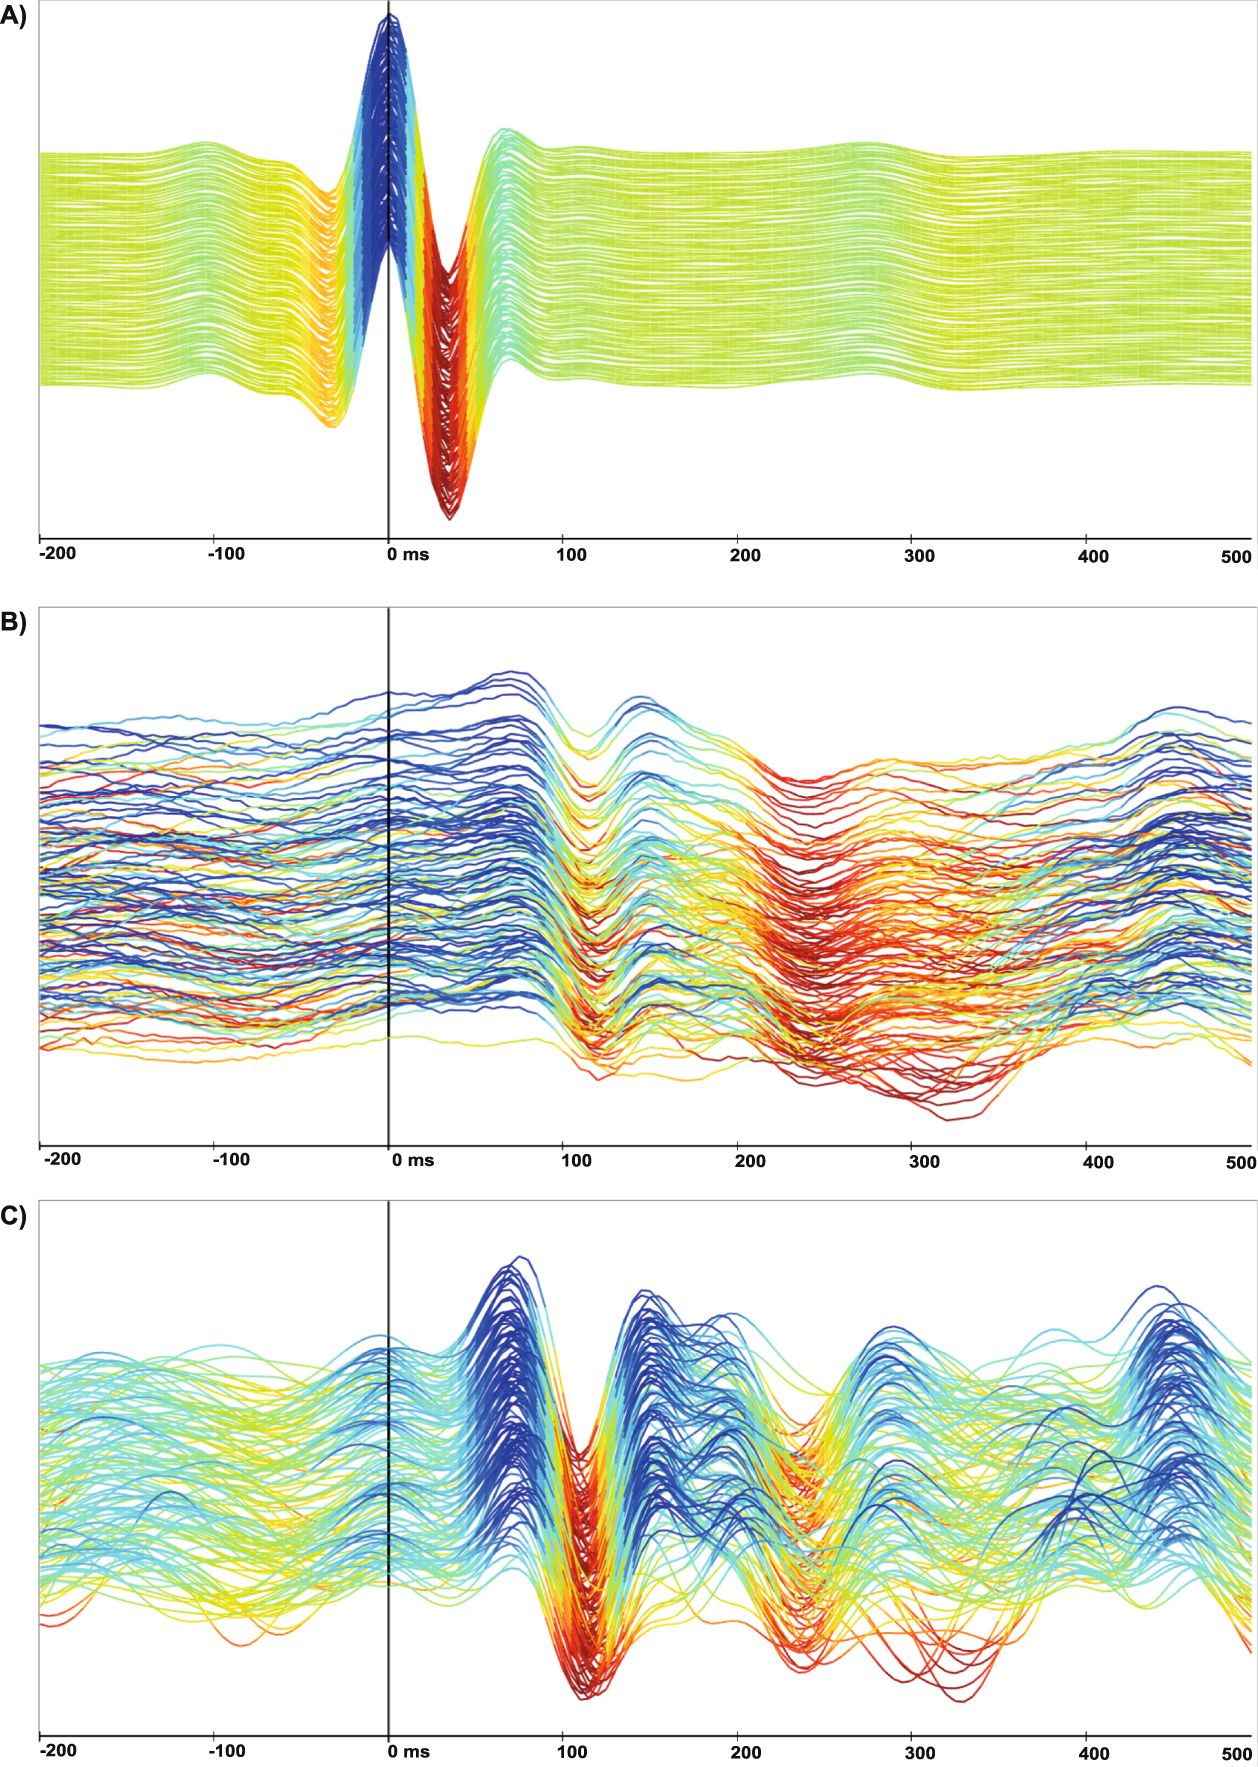
\includegraphics[width=0.5\textwidth]{pic/Variabilitaet.jpg}
		\caption[Visualisierung der Variabilität des \ac{BKG}-Signals]{Diagramm aus 128 konsekutiven Herzschlagen im EKG (A) und BKG (B,C), segmentiert durch das EKG. Die Farben dienen der besseren Visualisierung der Amplituden. (A) EKG-Signal; (B) BKG-Signal mit Überlagerungen durch Atmung und Bewegung; (C) \ac{BKG}-Signal ohne Bewegungsartefakte und Atmung.\protect\footnotemark}
		\label{fig:variabilitaet}
	\end{figure}
	\footnotetext{Entnommen aus \cite{Zink2017}.}
	
	
	Zusammengefasst lässt sich sagen, dass es sich bei ballistokardiographischen Signalen um nichtstationäre Signale handelt, dessen Ursprung nicht genau bekannt ist. Die Signalform wird von der Messachse, der Position und Körperhaltung der Proband*innen und dem Messsystem selbst beeinflusst. Besonders bei dem hier im Fokus liegenden Anwendungsfall Bett kommt es sowohl durch die unkontrollierbare Umgebung als auch die Signaleigenschaften selbst zu einer starken Variation der Morphologie und vielen Artefakten im Signal. Trotz dieser Einschränkungen ist die \acl{BKG} eine Messtechnik, die sich einfach \textit{unobtrusive} in den Alltag einbauen lässt und Aussagen über die \acl{HR} und die \acl{HRV} ermöglicht.

